\documentclass{article}
\usepackage[utf8]{inputenc}

\usepackage{amsmath}
\usepackage{hyperref}

\title{ECE220 Final Review - Cramming Carnival Solutions}
\author{Author: Members of HKN}
\date{Fall 2024}

\newcommand{\dd}[1]{\mathrm{d}#1}

\usepackage[makeroom]{cancel}
\usepackage[letterpaper, portrait, margin=1in]{geometry}
\usepackage{graphicx}
\usepackage{float}
\usepackage{enumitem}
\usepackage{graphicx}
\usepackage{multicol}
\usepackage{xcolor}
\usepackage{listings}

\definecolor{mGreen}{rgb}{0,0.6,0}
\definecolor{mGray}{rgb}{0.5,0.5,0.5}
\definecolor{mPurple}{rgb}{0.58,0,0.82}
\definecolor{backgroundColour}{rgb}{1,1,1}
\newcommand{\wideunderscore}{\underline{\hphantom{n}}}

\lstdefinestyle{CStyle}{
    backgroundcolor=\color{backgroundColour},   
    commentstyle=\color{mGreen},
    keywordstyle=\color{magenta},
    numberstyle=\tiny\color{mGray},
    stringstyle=\color{mPurple},
    basicstyle=\footnotesize,
    breakatwhitespace=false,         
    breaklines=true,                 
    captionpos=b,                    
    keepspaces=true,                 
    numbers=left,                    
    numbersep=5pt,                  
    showspaces=false,                
    showstringspaces=false,
    showtabs=false,                  
    tabsize=2,
    language=C,
    escapechar=\@
}

\pagenumbering{arabic}

\begin{document}

\maketitle

\section{
Logical Little Computer 3 Language Lessons}
\begin{enumerate}[label=(\alph*)]
    \item \textbf{I/O}: What is the difference between Polling I/O versus Interrupt I/O?
    \newline\textcolor{blue}{
    Polling I/O is when the program continually checks on the status of the input device (i.e. if a button has been pressed on the keyboard). Interrupt I/O is where the I/O device controls the flow, the device generates an “interrupt signal” which indicates that the device is ready with a new operation. The program gets “stuck waiting” in Polling I/O, but in Interrupt I/O the program continues until the interrupt signal is received.}

    \item \textbf{Stack}: When using a stack, when you pop an item off the stack, is it removed from memory?
    \newline\textcolor{blue}{When you pop an item off a stack, it is not actually removed from memory, instead the stack pointer is moved “down” to point to the next item on the stack.}
    
    \item \textbf{Stack Pt. 2}: If the input stream to a Stack is 123456789, design a set of pushes and Pops such that it is outputted 235641897?
    \newline\textcolor{blue}{push, push, pop, push, pop, push, push, pop, push, pop, pop, pop, push, push, pop, push, pop, pop
    This is the stack after each operation: \newline
    1, 21, 1, 31, 1, 41, 541, 41, 641, 41, 1, empty, 7, 87, 7, 97, 7,  empty, done.
    }
    \item \textbf{Subroutines}: What is the purpose of using subroutines in LC3?
    \newline\textcolor{blue}{ Subroutines allow you to break the code down into usable and resusable chunks that will be used multiple times so that you do not have to rewrite the same block of code each time. Example is the addition or multiplication subroutine for the stack calculator.
    }
    \item \textbf{Multiplication}: Write a Multiplication Subroutine in LC3 assembly language.
    \newline
    ;input R3, R4 \newline
    ;out R0 \newline
    MULTIPLY \newline
    ;your code goes here: \newline
    \newline\textcolor{blue}{
    ST R4, SaveR4    \hfill ; Callee-Save R4 \newline
    AND R0, R0, \#0   \hfill ; Clear R0 \newline
    MULTIPLY \newline
    ADD R0, R0, R3 \hfill \newline
    ADD R4, R4, \#-1 \hfill ; Decrement R4 \newline
    BRp MULTIPLY \hfill ; Loop Back if R4 is positive \newline
    \newline
    LD R4, SaveR4 \hfill ; Callee-Restore R4
    \newline
    RET
    \newline
    SaveR4 .BLKW \#1 \hfill ; Save this spot for R4}

    \item 
    \textbf{More subroutines}: What extra step do you need to take when executing a subroutine inside a subroutine? (Hint: What gets overwritten when JSR is called?)\newline
    \textcolor{blue}{ Save the value of R7 in memory so that you know which address to go back to in the original subroutine.}
    \end{enumerate}
    
\newpage
\section{Captivating C Coding}
\begin{enumerate}[label=(\alph*)]
    \item \textbf{Variable lifespan}: Explain the “lifespan” of a local variable during a C function call.
    \newline\textcolor{blue}{When a function gets called, the local variables are placed onto the runtime stack and are then used during the execution of the function. When the function returns control back to the main function the runtime stack pointer goes below the local variables so they are removed from the stack.
    }
    
    \item \textbf{Poopy Pointers}: Explain the importance of having the parameters of this function being pointers.
    
    \begin{lstlisting}[style=CStyle]
void swap(int* a, int* b)
{
    int temp;
    temp = *a;
    *a = *b;
    *b = temp;
} \end{lstlisting}

    \textcolor{blue}{Having parameters as pointers allow the data pointed to to actually change in the function. If the values were passed in as just their values, only the run time stack variables would be edited so that the operation would not be saved. Note how this function doesn't return anything.
    }
 
    \item \textbf{Lovely Linked Lists}: What is the benefit of using a linked list over an array to represent a large, ever-changing list?
    \newline\textcolor{blue}{It is significantly easier to both add and remove items in a linked list. Simply moving around some pointers makes it so that you can change the items easy.
    }
    \item \textbf{Rambunctious Recursion}: When writing a recursive algorithm, what is the goal of each recursive step? (Hint: The base case represents the simplest form of the problem)
    \newline\textcolor{blue}{The goal of each recursive step is to make the problem slightly simpler. An example is factorial, you calculate number * factorial(number-1). By decrementing the number each time, we make the problem easier, until we get to the base case.
    }
    \item \textbf{Arrays}: How are arrays passed into functions in C?
    \newline\textcolor{blue}{Arrays are passed as a pointer to the first item in the array. 
    }
    \item \textbf{Static Silliness}:  What is printed by the following program?
    \begin{lstlisting}[style=CStyle] 
static char letters[6] = {'A', 'E', 'F', 'D', 'B', 'C'};

void mystery () {
    static int X = 5;
    int Y = 2;
    printf ("%c%c", letters[--Y], letters[X--]);
}
int main() {
    mystery();
    mystery();
    return 0;
}
 \end{lstlisting}
    \textcolor{blue}{"ECEB" is printed; On the first call to mystery(), Y is set to 2 and X is statically set to 5. The notation "--Y" means to decrement, then use the result. "X--" means the opposite. So the first call to mystery() will print letters[1], letters[5], or "EC". Then the next call Y will be set back to 2. So it will print letters[1], letters[4], or "EB". Notice that X does not get set to 5 because it is declared as static, and does not get put on the stack, instead it is put in a different section of memory.
    }
    \newpage
    \item \textbf{Midpoint}: What is wrong with this recursive midpoint function?
\begin{lstlisting}[style=CStyle] 
find@\wideunderscore@midpoint(int a, int b) {
    if (a == b) { return a; }
    else if (a < b){
       return find_midpoint (a+1, b-1);
    } 
    else if (a > b){
       return find_midpoint( a-1, b+1); 
    } 
}\end{lstlisting}  
    \textcolor{blue}{There are two main things wrong. The first, is that were is no return type for this function, we need to make this return a float. The second, is that we need to deal with numbers that are odd-length apart, for example 4 and 7. To do this we can add: else if (a+1 == b) {return ((a+b)/2);} as another condition to check. }
    \item \textbf{Function Foo}: What is this function accomplishing? Assume it is called with a valid head to a singly linked list.
\begin{lstlisting}[style=CStyle] 
struct node{
    int num;
    struct node* next;
}
int foo(struct node* head, int bar) {
    if (head->num >= bar) {
        bar = head->num;
    }
    if (head->next == null) {
        return bar;
    }
    else {
        return foo(head->next, bar);
    }
}\end{lstlisting}  
    \textcolor{blue}{This function recursively returns the largest number of the linked list.}

\item Which sorting algorithm is this?
\begin{lstlisting}[style=CStyle]
void sort(int arr[], int n) {
    int i, j;
    for (i = 0; i < n - 1; i++)
        for (j = 0; j < n - i - 1; j++)
            if (arr[j] > arr[j+1])
                swap(&arr[j], &arr[j + 1]);
}\end{lstlisting}
\textcolor{blue}{This is bubble sort.}
    
    \item \textbf{Binary Search Trees}: Are these binary search trees?
    
    \includegraphics[width=7cm,height=6cm]{figures/bst.png}
    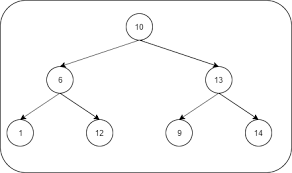
\includegraphics[width=7cm,height=6cm]{figures/notbst.png}
    
    \textcolor{blue}{Yes, No}
    \newpage
    \item \textbf{C to LC3}: Convert the following C function into LC3 using Callee Setup and Teardown.
    \begin{lstlisting}[style=CStyle] 
int foo(int a, int b) {
    int x;
    x = a + b;
    return x;
}\end{lstlisting}
    \textcolor{blue}{
    ADD R6, R6, \#-2 \hfill ; Allocate spot for return value\newline
    STR R7, R6, \#0    \hfill ; Push R7 (Return Address) \newline
    ADD R6, R6, \#-1  \newline
    STR R5, R6, \#0    \hfill ; Store R5 (Caller's Frame Pointer) \newline
    ADD R5, R6, \#-1 \hfill ;Set frame pointer for Callee \newline
    ADD R6, R6, \#-1 \hfill ;Allocate memory for local variables (x) \newline
    LDR R1, R5, \#4 \hfill ; Load a \newline 
    LDR R2, R5, \#5 \hfill ; Load b\newline
    ADD R0, R1, R2 \newline 
    STR R0, R5, \#0 \hfill ; Store result into x \newline
    STR R0, R5, \#3 \hfill ; Store result into return value slot \newline
    ADD R6, R5, \#1 \hfill ; Pop local variables\newline
    LDR R5, R6, \#0 \hfill ; Pop Frame Poitner\newline
    ADD R6, R6, \#1 \newline
    LDR R7, R6, \#0 \hfill ; Pop Return Address\newline
    ADD R6, R6, \#1 \newline
    RET
    \newline
}
    \item \textbf{Recursive Reversal}: What is the output of this program? If there is an error in ReverseArray, identify the line and fix it? (Hint: it might be nice and helpful to print every step of Reverse Array)
    
\begin{lstlisting}[style=CStyle] 
void ReverseArray(int array[], int size) {
    int start = 0;
    int end = size - 1;
    int temp;
    
    if (start < end) {
        // Swap First and Last
        temp = array[start];
        array[start] = array[end];
        array[end] = temp;
        
        ReverseArray(array, size-1);
    }
}
int main(){
    int array[5], i;
    for (i = 0; i<5; i++){
        array[i] = i;
    }
    ReverseArray(array, 5);
    printf("Reversed Array: ");

    for (i = 0; i<5; i++){
        printf("%d ", array[i]);
    }
    printf("\n");
    return 0;
}\end{lstlisting}

\textcolor{blue}{The program is basically just flipping the first and last elements, and then flipping the first and second to last and so on. So in the end, the only thing that actually changes is the first element goes to the front and the rest is shifted up. To fix this we need to change the recursive call to ReverseArray(array+1, size-2)}

\item \textbf{}What is wrong with the following code? 
\begin{lstlisting}[style=CStyle] 
double * firstlast(const double values[], int size)
{
    double result[2];
    result[0] = value[0];
    result[1] = value[size-1];
    return result;
}
\end{lstlisting}
\textcolor{blue}{The return value is a pointer to a local array that will go out of scope when the function ends, leading to an error.}

\item \textbf{Alternative Indexing}: Fill in the blanks to make the programs work properly.
\begin{lstlisting}[style=CStyle] 
int array1[4][2];
int array2[8];
int i, j;
for (i = 0; i < 2; i++) {
    for(j = 0; j < 4; j++) {
    array1[  ][  ] = i + j;
    array2[     ] = i + j;
    }
}
\end{lstlisting}
\textcolor{blue}{array1[i][j] \newline array2[(2*j) + i]}
\item Fill In the blanks to find the student with the highest GPA and store a pointer to them in best\_student
\begin{lstlisting}[style=CStyle] 
typedef struct StudentStruct {
    int UIN;
    float GPA;
} Student;

int main () {
    Student all_students[5];
    // Load data into all students:
    load_students(all@\wideunderscore@students, 5);
    // Find the student with the highest GPA:
    Student* best@\wideunderscore@student = 
    find@\wideunderscore@best(all@\wideunderscore@students, 5,         );
    printf("Best GPA:%f\n",         );
}

void find@\wideunderscore@best(Student* all, int num@\wideunderscore@students, Student** best) {
    for (int i = 0; i < num@\wideunderscore@students; i++) {
        if (all[i].GPA >        ) {
            // Fill:
        }
    }
}

\end{lstlisting}
\textcolor{blue} {
\&(all\_students[0])  \newline
\&best\_student   \newline
best\_student-$>$GPA  \newline
(*best)-$>$GPA  \newline
*best = \&(all[i]) \newline
}


\item In MP10, we tasked you with inserting a node into a sorted singly-linked list. To help you get accustomed to poopy pointer arithmetic, we will now attempt to do the same, but with a doubly-linked list. You are given the following struct doubly\_node and the function insert\_doubly\_node(), which takes in the head of a doubly linked list (but you will not have a tail) and a value to insert. Complete the function skeleton below. Assume that the double-pointer head is never NULL, but that the single pointer *head (the result of dereferencing head once) is not necessarily never NULL.

\begin{lstlisting}[style = CStyle]
    typedef struct doubly@\wideunderscore@node {
        int value
        doubly@\wideunderscore@node * next;
        doubly@\wideunderscore@node * prev;
    } doubly@\wideunderscore@node;


    void print@\wideunderscore@list@\wideunderscore@d(doubly@\wideunderscore@node * head)
    {
        doubly@\wideunderscore@node * cur = head;
        while (cur != NULL)
        {
            printf("%d -> ", cur->value);
            cur = cur->next;
        }
    }

    void insert@\wideunderscore@doubly@\wideunderscore@node(doubly@\wideunderscore@node ** head, int value) 
    {
        /* edge case 0: linked list is completely empty */
        if(*head ==   NULL      ) 
        {
            *head = ( doubly_node *  ) malloc(sizeof( doubly_node  ));
            (*head)->next =  NULL   ;
            (*head)->prev =   NULL   ;
            (*head)->value =  value   ;
            return;
        }

        /* edge case 1: insert AT the head*/
        if (value < (*head)->value      )
        {
            doubly@\wideunderscore@node * new_node = (doubly_node *   ) malloc(  sizeof(doubly_node) );
            new@\wideunderscore@node->value = value;
            new@\wideunderscore@node->next = *head; //new node should be inserted before head
            new@\wideunderscore@node->prev = NULL; //new node previous does not point to anything
            (*head)->prev  = new@\wideunderscore@node; //head's previous points to new@\wideunderscore@node
            *head = new_node; //update the new head of the linked list
            return;
        }

        doubly@\wideunderscore@node * cur = *head;
        while (cur != NULL     )
        {
            if (cur->value < value)
            {
                /* last edge case: insert AFTER the tail of the linked list */
                if (cur->next == NULL)
                {
                    doubly@\wideunderscore@node * new@\wideunderscore@node =   (doubly_node *) malloc(sizeof(doubly_node));                                ; 
                    //allocated new@\wideunderscore@node on the heap

                    new@\wideunderscore@node->value = value;
                    new@\wideunderscore@node->next = NULL; //new@\wideunderscore@node is the tail of the list
                    new@\wideunderscore@node->prev = cur; //new@\wideunderscore@node's previous points to the current
                    cur->next = new_node; //cur's next is the new node
                    return;
                }
                cur = cur->next;      // advance to the next node
            }
           

            else 
            {
                doubly@\wideunderscore@node * new@\wideunderscore@node = (doubly_node *  ) malloc(sizeof(doubly_node       ));
                new@\wideunderscore@node->value = value;
                new@\wideunderscore@node->next = cur;
                new@\wideunderscore@node->prev= cur->prev;
                cur->prev->next =  new_node;
                cur->prev = new_node;
                return;
            }
        }
    }
\end{lstlisting}

Assuming that insert\_doubly\_node() and print\_list\_d() are implemented correctly, what will the output of this code snippet be? 

\begin{lstlisting}[style = CStyle]
    int main()
    {
        doubly@\wideunderscore@node * head = NULL;
        insert@\wideunderscore@doubly@\wideunderscore@node(&head, 5);
        insert@\wideunderscore@doubly@\wideunderscore@node(&head, 2);
        insert@\wideunderscore@doubly@\wideunderscore@node(&head, 7)
        insert@\wideunderscore@doubly@\wideunderscore@node(&head, 9);
        insert@\wideunderscore@doubly@\wideunderscore@node(&head, 1);
        insert@\wideunderscore@doubly@\wideunderscore@node(&head, 10);
        insert@\wideunderscore@doubly@\wideunderscore@node(&head, 5);
        print@\wideunderscore@list@\wideunderscore@d(head);

        return 0;
    }
\end{lstlisting}

\textcolor{blue} {Answer:}
\begin{lstlisting}[style=CStyle]
1 -> 2 -> 5 -> 5 -> 7 -> 9 -> 10 ->
\end{lstlisting}

\end{enumerate}
\newpage
\section{C++ Programming}

\begin{enumerate}[label=(\alph*)]
    \item \textbf{Class}: What is the difference between structs in C and classes in C++?
    \newline\textcolor{blue}{Both structs in C and classes in C++ have the ability to define the data inside of the class/struct. However,  classes in C++ have two extra things. Classes have the ability to control “security” in which you can determine who can access certain parts. Classes also allow you can to define functions that are specific to the class.}
    \item \textbf{Constructor}: What does a constructor do in a class? What does a destructor do in a class? What might happen if we do not have a correct destructor?
    \newline\textcolor{blue}{A constructor is a special member function that creates and initializes a new object. A destructor is a special member function that deletes an object and free’s all dynamically allocated memory. If destructor is not implement or implemented incorrectly, there might be memory leak since there are memories not being freed}
    \item \textbf{Access specifier}: What is the difference between public, private, and protected in a C++ class?
    \newline\textcolor{blue}{Public members can be accessed by anyone who accesses the class. Private members can only be accessed by member functions. Protected members are similar to private as it can only be accessed by member function, but it can be used in member functions of classes derived from the class (Inheritance).}
    \item What does operator overloading do in a C++ class? Give four different examples of operators that can be overloaded.
    \newline\textcolor{blue}{Overloading an operator allows you to redefine the built in operators, including +, -, *, <, >, =, to allow them to work with your user defined classes}
    \item \textbf{Rectangle}: Write the constructors and area function for this rectangle class.
    \begin{lstlisting}[style=CStyle]
class Rectangle {
private:
    int width, height;
public:
    Rectangle();
    Rectangle(int w, int h);
    int const area();
}
\end{lstlisting}
\textcolor{blue}{Answer:}
\begin{lstlisting}[style=CStyle]
Rectangle::Rectangle() {
    width = 0;
    height = 0;
}

Rectangle::Rectangle(int w, int h) {
    width = w;
    height = h;
}

int Rectangle::area() const {
    return width * height;
}\end{lstlisting}

\textcolor{blue}{Why initialize width and height to 0 and not 1?. Also  we could use $\rightarrow{}$ to reference member variables}
    \item \textbf{Iterator}: What will be printed if we run the following C++ code? (assume we import all needed files)
    \begin{lstlisting}[style=CStyle]
    int main() 
{ 
    vector<int> ar = { 1, 2, 3, 4, 5 }; 
    vector<int>::iterator ptr = ar.begin(); 
    ptr++;
    cout << *ptr << endl; 
    ptr = ptr + 3;
    cout << *ptr << endl; 
    return 0; 
}
\end{lstlisting}
\textcolor{blue}{2 and 5 will be printed. When initializing the iterator to begin(), it is at the first position. ++ will move the iterator to the second position and printed 2. + 3 will move the iterator to 3 positions later, which is at 5}
    \item \textbf{Template}: What will happen if we run the main function?
    \begin{lstlisting}[style=CStyle]
template <typename T>
T max(T x, T y)
{
    return (x > y)? x : y;
}
int main()
{
    cout << max(3, 7) << endl;
    cout << max(3.0, 7.0) << endl;
    cout << max(3, 7.0) << endl;
    return 0;
}
\end{lstlisting}
\textcolor{blue}{Nothing will be printed because an error is caused at line 10. A template can be used so that we can use one function with different types, so the max function works at lines 8 and 9 since the function can both accept int and float. However, at line 10, we pass one int and one float into the function, which are different types. This generates a compiler error because of the ambiguity.}
    \item \textbf{Copy}: What is the difference between shallow copy and deep copy?
\newline\textcolor{blue}{Shallow copy only copies the variables of the original object. If one of the variables is a pointer, it will only copy the pointer but not the data it points to, so they are still pointing to the same data. But deep copy will not only copy the variables but allocate similar memory with the same value as the original object. So the data the pointers point to will also be copied in newly allocated memory}

    \item \textbf{} What type of traversal is this?
    \begin{lstlisting}[style=CStyle]
void traversal (node *root) {
    if ( root != NULL) {
       std::cout << root -> data << std::endl;
       traversal (root -> left);
       traversal (root -> right);
    }
 }
    \end{lstlisting}
    
\textcolor{blue}{This is an example of Pre-Order traversal. This algorithm will recursively iterate through the nodes in the tree, starting at the root and traversing to the left and the right subtrees respectively.}

    \item \textbf{}
What is the pre-order, in-order, post-order and level order traversal for the following binary search tree?

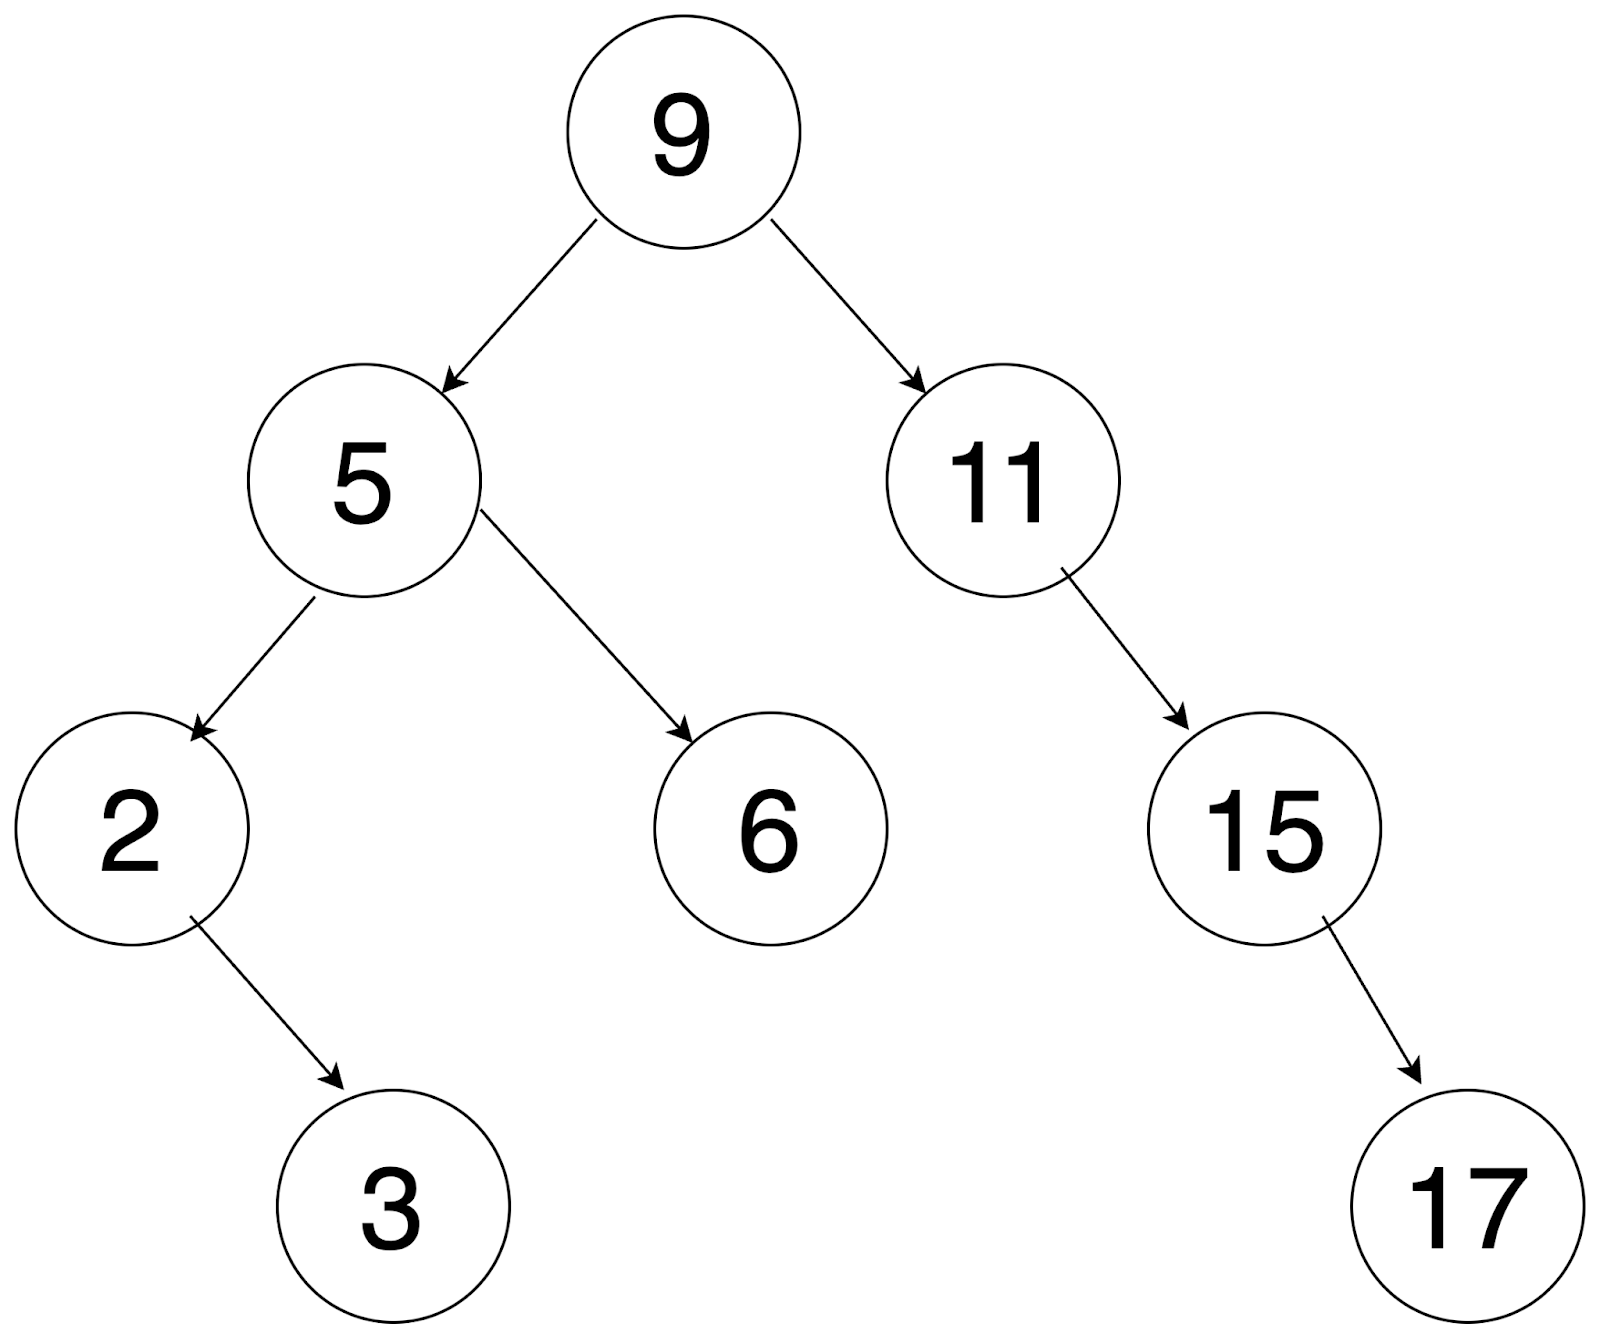
\includegraphics[scale = 0.125]{figures/bst2.png}\newline
\textcolor{blue}{Pre-Order: 9, 5, 2, 3, 6, 11, 15, 17}\newline
\textcolor{blue}{In-Order: 2, 3, 5, 6, 9, 11, 15, 17}\newline
\textcolor{blue}{Post-Order: 3, 2, 6, 5, 17, 15, 11, 9}\newline
\textcolor{blue}{Level-Order: 9, 5, 11, 2, 6, 15, 3, 17}\newline
\item \textbf{}
How many bytes of memory have been allocated on the heap? Assume that we are in a 32-bit system (recall that an int is 4 bytes, a double is 8 bytes, an int * is 4 bytes, and a char is 1 byte)

    \begin{lstlisting}[style=CStyle]

    int main () {
        int a = 4;
        int d = 6;
        int c = 10; 
        int ** b = new int * [5];  
        b[0] = &a;
        b[1] = &c;   
        b[2] = &d;
        b[3] = new int[6];
        b[3][0] = 5;
        b[3][2] = 8;
        b[3][1] = 17;
        b[3][5] = 2;
        b[3][4] = 9;
        b[3][3] = 22; 
        b[4] = new int(13);
        char * character = new char (k);
 }


    \end{lstlisting}

    \textcolor{blue} {20 + 24 + 4 + 1 = 49 bytes}

    Write the contents of what each pointer points to (if it points to an array, write the contents of the array. If it points to a single int/char, write what the int/char is.) \newline
    \textcolor{blue} 
{ 4 \\
10\\
6\\
5 17 8 22 9 2\\
13\\
k\\
}

Fill in the lines after line 10 needed to properly free the memory. Not all lines may be needed.

    \begin{lstlisting}[style=CStyle]
int main () {
    int a = 4;
    int d = 6;
    int c = 10;
    int ** b = new int * [5];  
    b[0] = &a;
    b[1] = &c;   
    b[2] = &d;
    b[3] = new int[6];
    b[3][0] = 5;
    b[3][2] = 8;
    b[3][1] = 17;
    b[3][5] = 2;
    b[3][4] = 9;
    b[3][3] = 22; 
    b[4] = new int(13);
    char * character = new char('k');
    @\textcolor{blue}{delete [] b[3];}@
    @\textcolor{blue}{delete b[4];}@
    @\textcolor{blue}{delete [] b;}@
    @\textcolor{blue}{delete character;}@
 }

    \end{lstlisting}

    Let’s say we have a void pointer p. What is the difference between delete [] p and delete p?

    \textcolor{blue}{ delete [] will free a contiguous array of memory, while delete frees only a single allocated block of memory of a particular data type. (e.g, an array of ints vs. a single int) }

    \item Linked List Problem:
    Your best friend Gabriel has a C program that stores the name of his favorite Fortune 500 company. He is storing the company name in a linked list format. The structure of the linked list and the nodes are located below. The end of the list will have the company\@\wideunderscore\@node * next point to NULL;

    \begin{lstlisting}[style = CStyle]
        typedef struct company@\wideunderscore@node
        {
            int index;
            char letter;
            struct company@\wideunderscore@node * next;
            
        } company@\wideunderscore@node;

        typedef struct company
        {
            int n; //number of entries in list
            company@\wideunderscore@node * company_head;
            
        } company;
    \end{lstlisting}

    Given the above structure, and the fact that the company\wideunderscore node * pointer is 8 bytes (64-bit system),
    \textbf{what is the size in bytes of both struct company and struct company\wideunderscore node?}
    \newline\textcolor{blue}{company: 4 + 8 = 12 bytes}
    \newline\textcolor{blue}{company\@\wideunderscore\@node: 4 + 1 + 8 = 13 bytes}

    \vspace{2.5cm} %adding space for student answer
    
    Gabriel wants to tell you what his favorite Fortune 500 company is but is unable to speak because he just got his wisdom teeth removed. \textbf{Fill in the below program to print the name of the company.} This program takes place in main and has already imported the relevant libraries. 

    Assume everything has been initialized/malloc'd correctly and the name of the struct was declared with the following line. 

    Part 1: Printing

    \begin{lstlisting}[style = CStyle]
        company * gabriel@\wideunderscore@company;

        printf("The Name of Gabriel's Favorite Fortune 500 Company: ");

        company@\wideunderscore@node * current = gabriel@\wideunderscore@company->company@\wideunderscore@head;
        for (int i = 0; i < @\textcolor{blue}{gabriel\wideunderscore\@company-$>$n}@; i++) // iterate through the list
        { 
            printf("%c", @\textcolor{blue}{current-$>$letter}@); //print the current character
            @\textcolor{blue}{current = current-$>$next}@; //move the current node
        }
    \end{lstlisting}
    
    Gabriel is quite shy and doesn't want anyone to know what his favorite Fortune 500 company is (except for you, his best friend). \textbf{Help him finish the below code to remove the company name from the heap.}

    Part 2: Freeing
    \begin{lstlisting}[style = CStyle]
        company@\wideunderscore@node * the@\wideunderscore@current = gabriel@\wideunderscore@company->company@\wideunderscore@head;
        company@\wideunderscore@node the@\wideunderscore@previous = gabriel@\wideunderscore@company->company@\wideunderscore@head;
        while(the@\wideunderscore@current->next != @\textcolor{blue}{NULL}@  ){
            the@\wideunderscore@current = the@\wideunderscore@current->next;
            free(@\textcolor{blue}{the\wideunderscore previous}@);
            @\textcolor{blue}{the\wideunderscore previous = the\wideunderscore{current} }@; //move previous further
        }

        free(gabriel@\wideunderscore@company);
    \end{lstlisting}

    Whenever the above code is executed, a memory leak occurs. 
    \textbf{Explain what a memory leak is and come up with one line of code that can be added above to fix the memory leak.}\newline

    \textcolor{blue}{A memory leak is when we forget to free allocated memory or lose access to a region of allocated memory due to a pointer value being changed. We can fix this by revising line 8 as follows:}

    \begin{lstlisting}[style=CStyle]
    company@\wideunderscore@node * the@\wideunderscore@current = gabriel@\wideunderscore@company->company@\wideunderscore@head;
        company@\wideunderscore@node the@\wideunderscore@previous = gabriel@\wideunderscore@company->company@\wideunderscore@head;
        while(the@\wideunderscore@current->next != @\textcolor{blue}{NULL}@  ){
            the@\wideunderscore@current = the@\wideunderscore@current->next;
            free(@\textcolor{blue}{the\wideunderscore previous}@);
            @\textcolor{blue}{the\wideunderscore previous = the\wideunderscore{current} }@; //move previous further
        }
        @\textcolor{blue}{free(the\wideunderscore current)}@;
        free(gabriel@\wideunderscore@company);
    \end{lstlisting}

    
    
    \item Virtual Keywords:
    \begin{lstlisting}[style = CStyle]
        #include <iostream>
        class Base
        {
            public: 
                virtual void f()
                {
                    std::cout << "base\n";
                }
        };

        class Derived@\wideunderscore@One : public Base
        {
            public:
                void f() override
                {
                    std::cout << "derived_1\n";
                }
        };

        class Derived@\wideunderscore@Two : public Base 
        {
            public: 
                void f()
                {
                    std::cout << "derived_2\n";
                }
        };

    
        int main()
        {
            //Define the objects
            Base b;
            Derived@\wideunderscore@One d@\wideunderscore@1;
            Derived@\wideunderscore@Two d@\wideunderscore@2;

            //assign the objects by reference
            Base& br = b;
            Base& dr@\wideunderscore@1 = d@\wideunderscore@1;
            Base& dr@\wideunderscore@2 = d@\wideunderscore@2;

            /* PART 1 */
            br.f();
            dr@\wideunderscore@1.f();
            dr@\wideunderscore@2.f();

            //Assign the objects by pointer
            Base * bp = &b;
            Base * dp_1 = &d@\wideunderscore@1;
            Base * dp_2 = &d@\wideunderscore@2;

            /* Part 2 */
            bp->f();
            dp@\wideunderscore@1->f();
            dp@\wideunderscore@2->f();

            /* Part 3 */
            br.Base::f();
            dr@\wideunderscore@1.Base::f();
            dr@\wideunderscore@2.Base::f();

            return 0
        }
    \end{lstlisting}
    Part 1:
    What is printed by br, dr\_1, and dr\_2?
    \newline\textcolor{blue}{base}
    \newline\textcolor{blue}{derived\@\wideunderscore\@1}
    \newline\textcolor{blue}{derived\@\wideunderscore\@2}
    
    \vspace{2cm}
    Part 2:
    What is printed by br, dr\_1, and dr\_2? What is the difference between Part 1 and Part 2?
    \newline\textcolor{blue}{base}
    \newline\textcolor{blue}{derived\@\wideunderscore\@1}
    \newline\textcolor{blue}{derived\@\wideunderscore\@2}
    
    \vspace{1cm}
    
\textbf{Note}: \textcolor{blue}{In Part 1, we accessed the functions through objects by reference. In Part 2, we accessed the functions through objects by pointers.}

    \vspace{2cm}
    Part 3:
    What is printed br, dr\_1, and dr\_2? What is the difference between the other two parts?
    \newline\textcolor{blue}{base}
    \newline\textcolor{blue}{base}
    \newline\textcolor{blue}{base}
    \vspace{2cm}
    \end{enumerate}

\textbf{Note}: \textcolor{blue}{In Part 1 and Part 2, we default to the virtual functions despite the objects being a type “Base”. With Part 3, we explicitly ask for the parent version of the function through Base::f().}




    

\end{document}